\documentclass[10pt,a4paper,onecolumn,titlepage]{article}
\usepackage[utf8]{inputenc}
\usepackage[croatian]{babel}
\usepackage{amsmath}
\usepackage{amsfonts}
\usepackage{amssymb}
\usepackage{graphicx}
\usepackage{hyperref}

\title{Višekorisnička chat aplikacija u C\#-u}
\author{Antonio Kovačić\\Janko Marohnić\\Lana Arzon}

\begin{document}
\maketitle

\tableofcontents

\newpage

\section{Opis problema}

Potrebno je napraviti aplikaciju za gdje se ljudi mogu međusobno dopisivati
u realnom vremenu. Dvije ili više osoba se treba moći "naći na jednom mjestu",
i komunicirati zajedno putem tekstualnih poruka.

Kada se osoba prijavi u chat, treba upisati svoje korisničko ime, kojim će se
ta osoba identificirati. Ako je postoji druga osoba u istoj "sobi" koja već
ima željeno korisničko ime, osoba bi trebala izabrati drugo korisničko ime.
Nakon što je upisala korisničko ime, osoba mora moći vidjeti koji su sve drugi
korisnici trenutno prijavljeni u istu "sobu".

Kada osoba pošalje poruku u grupni chat (napiše teskt i stisne "enter"), svaka
druga osoba mora primiti tu istu poruku (i treba pisati od koga dolazi). Na taj
način svatko zna što su svi ostali rekli. I poruke moraju stizati redom kojim
su poslane.

Kada se osoba odjavi iz chata, ostalim osobama treba doći poruka da se ta
osoba odjavila iz chata.

\section{Implementacija}

\subsection{Server}

\subsubsection{Kreiranje}

\subsubsection{Instaliranje}

\subsubsection{Pokretanje}

\begin{figure}[!ht]
\begin{minipage}{\textwidth}
\centering
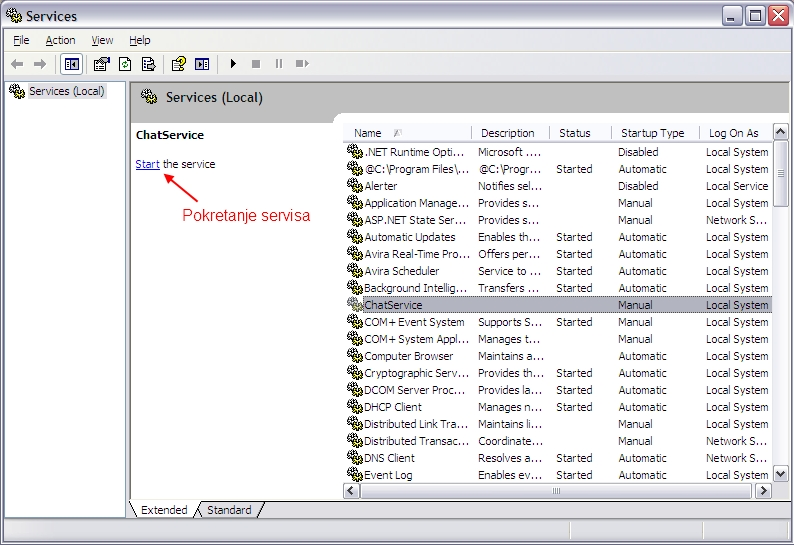
\includegraphics[width=\textwidth]{images/start_service.jpg}
\caption{Pokretanje servisa ChatService}
\end{minipage}
\end{figure}

\subsection{Klijent}

U klijentu nalazimo TCP kanal servisa, i spojimo se na server. Ako servis
nije upaljen, javljamo grešku.

Zatim ispisujemo poruku dobrodošlice, i vadimo sa servisa sve trenutno prijavljene
korisnike, i ispisujemo njihova korisnička imena novopridošlom korisniku. 

\begin{figure}[!ht]
\begin{minipage}{\textwidth}
\centering
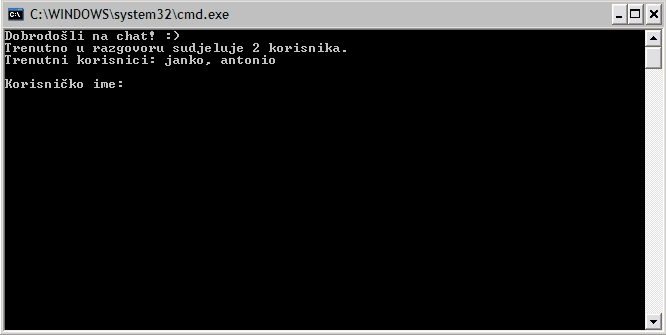
\includegraphics[width=\textwidth]{images/welcome.jpg}
\caption{Poruka dobrodošlice, broj prijavljenih korisnika i ispis njihovih korisničkih imena}
\end{minipage}
\end{figure}

Zatim ga tražimo da upiše svoje korisničko ime, s time da server provjerava postoji li
već korisničko ime, i u tom slučaju traži korisnika da upiše drugo korisničko ime.

\begin{figure}[!ht]
\begin{minipage}{\textwidth}
\centering
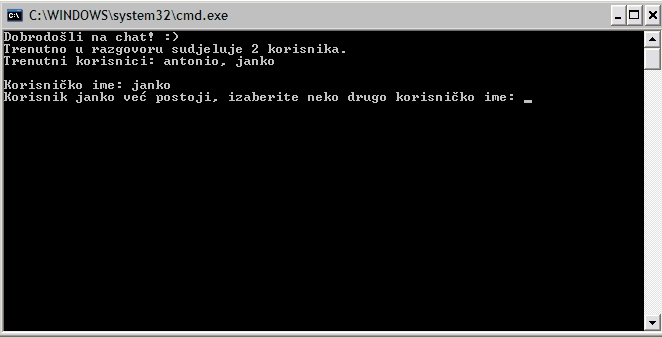
\includegraphics[width=\textwidth]{images/invalid_username.jpg}
\caption{Nemogućnost unosa već postojećeg korisničkog imena}
\end{minipage}
\end{figure}

Također, unos korisničkog imena je obavezan pa ako ga nismo unijeli, dobivamo upozorenje da to moramo učiniti.

\begin{figure}[!ht]
\begin{minipage}{\textwidth}
\centering
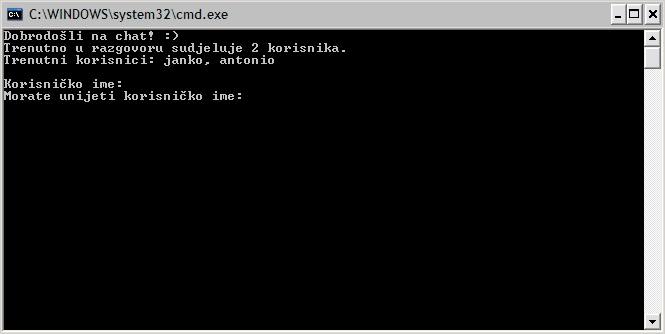
\includegraphics[width=\textwidth]{images/username_required.jpg}
\caption{Unos korisničkog imena je obavezan}
\end{minipage}
\end{figure}

Nakon prijave se svim korisnicima šalje obavijest da se novi korisnik prijavio
u chat, i korisnik se dodaje u servis.

\begin{figure}[!ht]
\begin{minipage}{\textwidth}
\centering
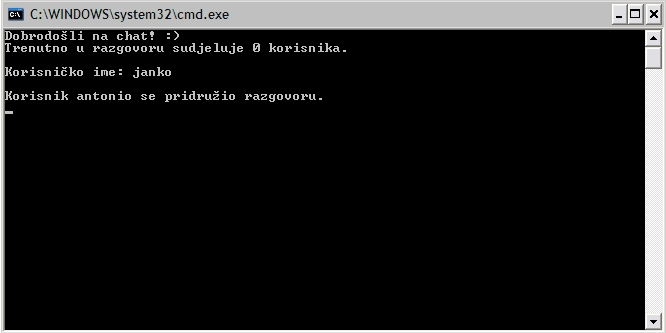
\includegraphics[width=\textwidth]{images/joining_notification.jpg}
\caption{Korisnik se pridružje razgovoru}
\end{minipage}
\end{figure}

Komunikacija se odvija na način da korisnik unese poruku koju zatim server prosljeđuje svim ostalim korisnicima koji su prijavljeni na chat.

\newpage

\begin{figure}[!ht]
\begin{minipage}{\textwidth}
\centering
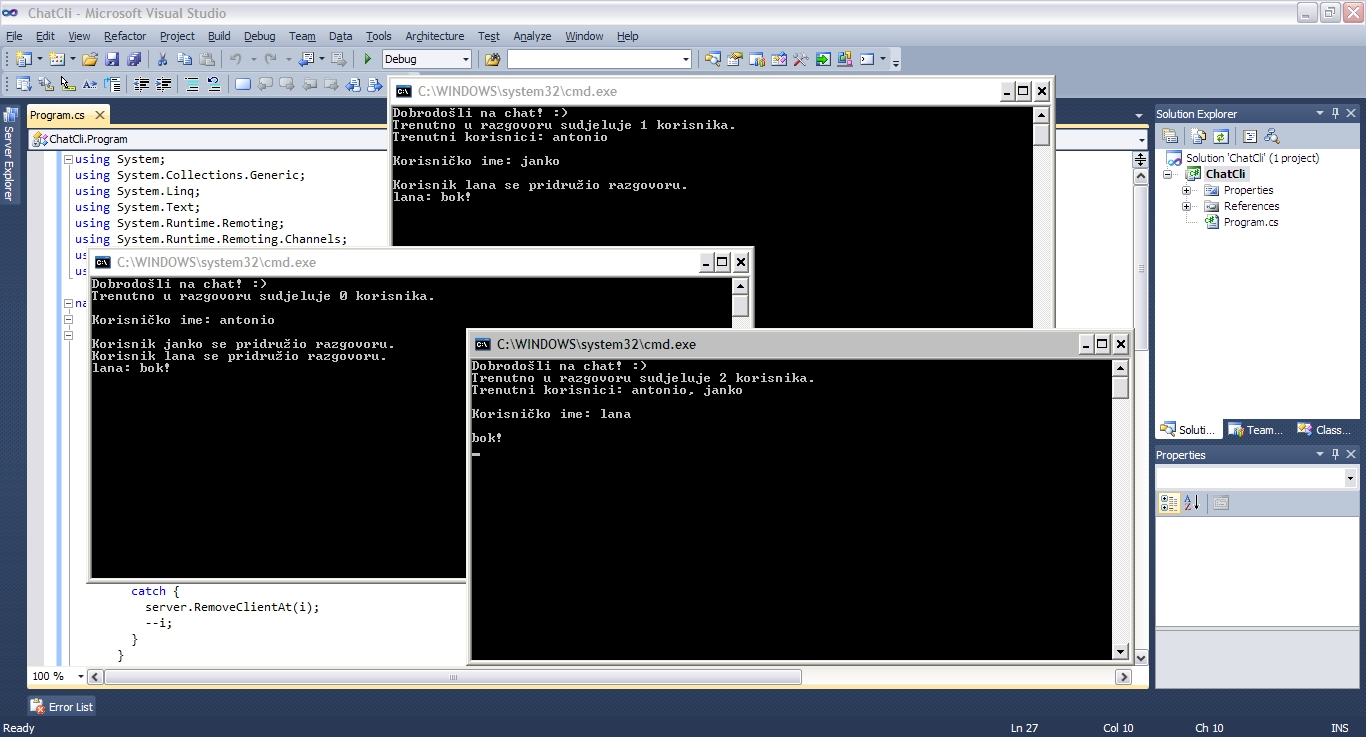
\includegraphics[width=\textwidth]{images/comunication.jpg}
\caption{Primjer jednostavne komumnikacije}
\end{minipage}
\end{figure}

Korisnik može u bilo kojem trenutku napustiti razgovor te nakon što to učini, svi ostali korisnici dobivaju obavijest o tome.

\begin{figure}[!ht]
\begin{minipage}{\textwidth}
\centering
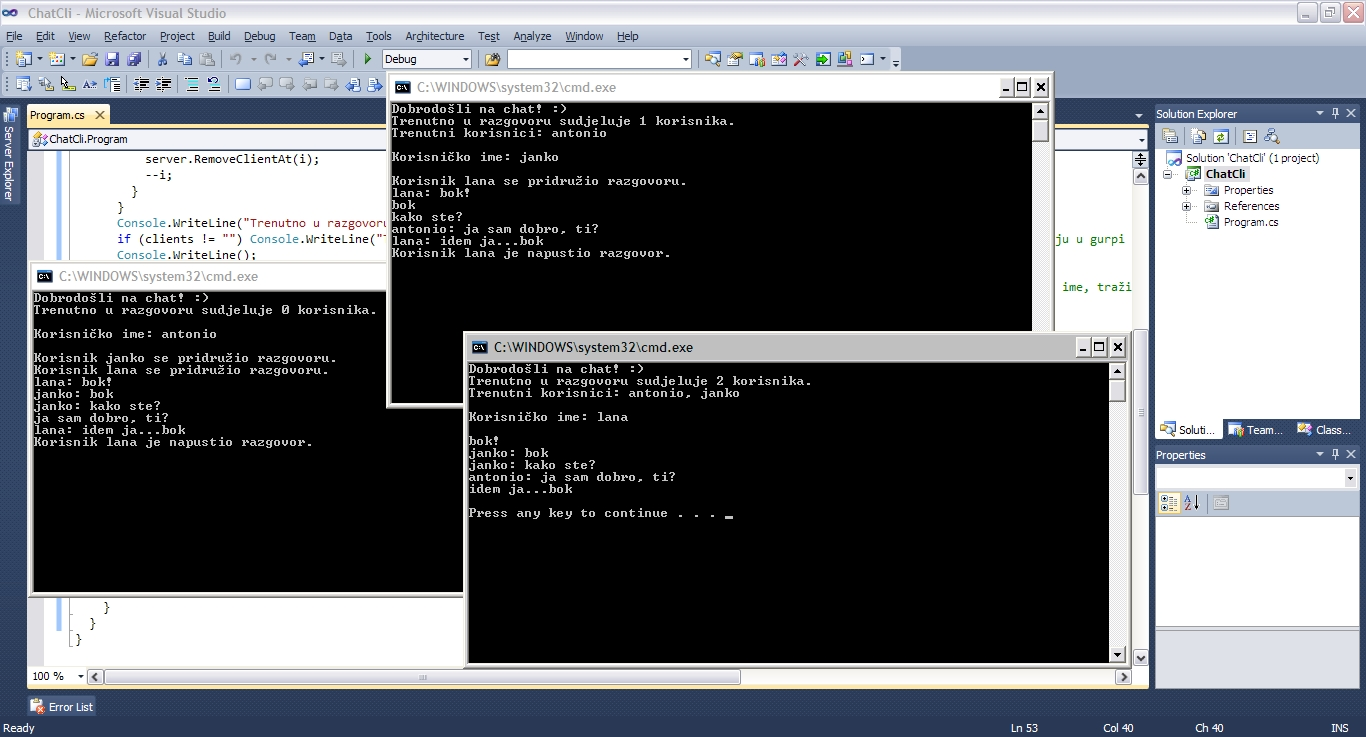
\includegraphics[width=\textwidth]{images/leaving_notification.jpg}
\caption{Korisnik napušta razgovor}
\end{minipage}
\end{figure}

\section{Rasprava}

Ova implementacija ima nekoliko prednosti. Jedna je da smo koristili Windowsove
servise za server, umjesto da smo implementirali svoj vlastiti. Na taj način
možemo biti sigurni da je taj server optimiziran i za veći broj korisnika.
Druga je što danas programeri uglavnom provode vrijeme u komandnoj liniji,
pa činjenica da je naša chat aplikacija napisana kao komandno-linijska aplikacija
pruža takvim korisnicima već poznato okruženje. Treća prednost je to što kada
zgasimo računalo, ugasi nam se i servis, pa nemamo problema sa eventualnim
cachiranjem koje bi druge implementacije mogle napraviti.

Neke mane naše implementacije su da, ukoliko korisnik zgasi prozor, naš servis
ne registrira da se korisnik odjavio (jer je zapravo došlo do iznimke, a naš
program trenutno ne obrađuje tu iznimku). Druga mana je da kada korisnik
piše poruku, a u isto mu vrijeme stigne poruka od nekog drugog korisnika,
zbog ograničenja komandne linije će mu pisanje vizualno prekinuti novopristigla
poruka. Korisnik još uvijek može dovršiti svoju poruku, i normalno je poslati,
samo mu se može učiniti da je došlo do greške.

\end{document}
